%__________________________________________________________________________________

\chapter{Local-Timed Negotiations}
\label{chap:ltn}

The previous chapters developed two complementary viewpoints on concurrency and
time: negotiations make causality and independence explicit through interaction
structure, while timed automata capture quantitative timing through clocks and
guards.  This chapter combines those viewpoints without collapsing distributed
behaviour onto a single global timeline.  We introduce \emph{local-timed
negotiations} (LTNs), in which each agent carries its own local time, time
elapses independently for different agents, and equality of local times is
imposed only at explicitly chosen interaction points.

The chapter has two goals. The first is modelling: LTNs provide a natural
formalism for local deadlines, response windows, and selectively synchronized
coordination in distributed systems.  The second is algorithmic: the combination
of local drift and explicit synchronization already yields a model whose
location-reachability problem is undecidable.  This boundary result motivates
the decidable fragments studied in Part~II.

\section{Motivation: Why Local Time?}

\paragraph{The inadequacy of global time.} Networks of timed automata (Section~\ref{sec:networks-ta}) assuming \emph{global time}, i.e., all clocks advance uniformly during delay transitions, and synchronization is instantaneous is inadequate to represents distributed reality for three main reasons:

\begin{itemize}
  \item \textbf{Local clocks:} in realistic distributed protocols, agents progress
        at different rates due to clock drift, computation time, and network
        delays.
  \item \textbf{Partial synchrony:} real systems combine tightly synchronized
        interactions with loosely coupled, independent computation.
  \item \textbf{Agent-centric timing:} timing constraints are often relative to an
        agent’s own actions (e.g.\ completing a workflow within a fixed time after
        initiation), which is awkward to express using a single global timeline.
\end{itemize}

\paragraph{The local-time perspective.} Local-timed negotiations adopt a fundamentally different view: each agent $p$ has a \emph{reference clock} $t_p$ that measures its local elapsed time. Between interactions, agents progress independently—one agent may experience 5 time units while another experiences only 2. At interactions (negotiation nodes), agents coordinate by selecting outcomes that respect their local clock constraints (guards). 

Crucially, LTNs introduce \emph{explicit synchronization} as a modeling choice:
selected nodes may require that participating agents’ reference clocks are equal
when the interaction occurs.  This captures scenarios where coordination demands
temporal alignment, such as simultaneous authentication or tightly coupled sensor
fusion.

\paragraph{What we gain.} This synthesis yields several benefits:

\begin{itemize}
\item \textbf{Explicit concurrency}: The negotiation structure makes independence and causality transparent. Actions involving disjoint agents can occur concurrently without artificial interleaving.

\item \textbf{Agent-centric timing}: Each agent tracks its own deadlines, timeouts, and response times via local clocks, more naturally modeling distributed systems than shared global clocks.

\item \textbf{Selective synchronization}: Synchronizing nodes explicitly capture coordination points where temporal alignment matters, while unsynchronized nodes allow agents to drift.

\item \textbf{Rich expressiveness}: As we'll see, LTNs can model behaviors impossible in purely global-time or purely asynchronous settings, including causal enforcement through timing and non-regular untimed languages.
\end{itemize}

\paragraph{What we sacrifice.} This expressiveness comes at a cost: \emph{unrestricted LTNs have undecidable reachability}. The combination of unbounded clock drift and explicit synchronization creates computational power equivalent to counter machines. The remainder of this thesis identifies restrictions that recover decidability while preserving modeling advantages.

\paragraph{Chapter roadmap.} Section~\ref{sec:ltn-example-informal} motivates the model through a running ATM
example.  Section~\ref{sec:ltn-def} formalizes LTNs, and
Section~\ref{sec:ltn-semantics} gives their operational semantics.
Section~\ref{sec:ltn-related} positions the model with respect to related timed
extensions of negotiations and to local-time semantics for timed automata.
Section~\ref{sec:ltn-expressiveness} illustrates two characteristic
expressiveness phenomena, and Section~\ref{sec:ltn-undec} proves undecidability
of location-reachability.  Section~\ref{sec:summary-ch3} distils the main
message of the chapter and prepares the transition to Part~II.

%---------------------------------------------------------------------------------

\section{Related work}
\label{sec:ltn-related}

Negotiations were introduced by Esparza et al.~\cite{DBLP:conf/concur/EsparzaD13,DBLP:journals/acta/DeselEH19}
and admit efficient analysis for several subclasses~\cite{DBLP:journals/lmcs/EsparzaKMW18,DBLP:conf/lics/EsparzaMW17}.
Timed negotiations, which associate durations with outcomes of atomic
negotiations, were studied in~\cite{DBLP:conf/fossacs/AkshayGHM20}; we provide a
detailed comparison with LTNs below.

Local-time semantics for networks of timed automata originates
in~\cite{DBLP:conf/concur/BengtssonJLY98} and has recently been used for
zone-based verification~\cite{DBLP:conf/concur/GovindHSW19,DBLP:conf/lics/0001HSW22}
and B\"uchi reachability~\cite{DBLP:conf/concur/HerbreteauSW22}.  In contrast to
NTA, where shared actions enforce synchronization by design, LTNs start from a
local-time view and offer synchronization as a modeling choice.

\subsection{Comparison with Timed Negotiations~\cite{DBLP:conf/fossacs/AkshayGHM20}}
\label{subsec:ltn-vs-tn}

Timed negotiations~\cite{DBLP:conf/fossacs/AkshayGHM20} extend negotiations
by associating durations with outcomes of atomic negotiations.
Time progress is modelled by assigning durations to individual interactions,
which determine when subsequent negotiations become available.

In contrast, LTNs adopt a clock-based semantics inspired by timed automata,
where time elapses independently of interactions and can be constrained
across multiple negotiations.  This difference has several consequences.
First, LTNs can naturally express timing constraints that relate distinct
interactions, such as deadlines or response-time constraints spanning an
entire workflow.  Second, LTNs allow agents to accumulate and compare local
time through explicit synchronization nodes, whereas timed negotiations
lack a mechanism for comparing temporal progress across interactions.

From an algorithmic perspective, these additional features strictly
increase expressive power: as shown in Section~\ref{sec:ltn-undec},
location-reachability is undecidable for LTNs, whereas timed negotiations
retain decidability for basic analysis problems.  This contrast highlights
the trade-off between expressiveness and tractability when extending
negotiations with time.

Viewed together, timed negotiations and LTNs represent complementary
points in the design space: the former favor tractable timing of
individual interactions, while the latter prioritize expressive,
agent-centric temporal reasoning across interactions.

%---------------------------------------------------------------------------------

\section{Introducing Local-Timed Negotiations: An Informal Example}
\label{sec:ltn-example-informal}

Before formal definitions, we introduce LTNs through an extended version of the ATM transaction example from Chapter~\ref{chap:preliminaries}, now enhanced with timing constraints.

\subsection{Scenario: ATM Transaction with Timeouts}

Recall the basic workflow: a customer ($c$) resets their ATM PIN using a one-time password (OTP) sent by the bank ($b$) through the ATM machine ($a$). We now add realistic timing requirements:

\begin{enumerate}
\item \textbf{Customer timeout}: The customer wants the entire transaction (from request to completion) to take at most 10 time units. If this deadline is exceeded, the customer gives up.

\item \textbf{Bank security policy}: The bank requires that at most 3 time units elapse between sending the OTP and validating it (to prevent replay attacks). Failed validation attempts must also respect this 3-unit window.

\item \textbf{Local time progression}: The customer, ATM, and bank may experience different amounts of elapsed time between interactions due to processing delays, network latency, or user hesitation.
\end{enumerate}

\subsection{Modeling with Local Clocks}

Figure~\ref{fig:ATM} depicts this scenario as a local-timed negotiation. The basic structure follows the untimed negotiation from Chapter~\ref{chap:preliminaries}, augmented with timing annotations:

\begin{figure}[t]
  \centering
  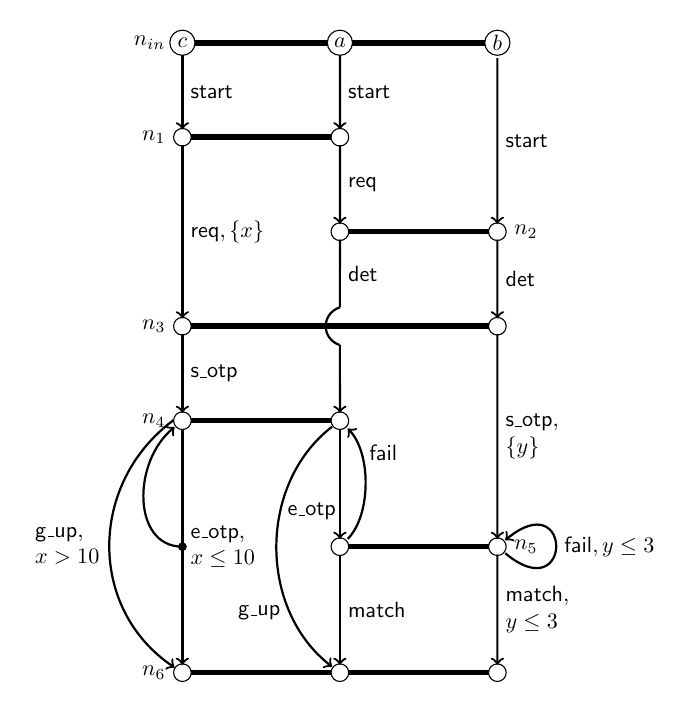
\begin{tikzpicture}[scale=0.8, every node/.style={transform shape}]

\begin{scope}[line width=2pt]
  \draw (0.,0) node [left] {$n_{\text{in}}\,\,$} -- (5,0); 
  \draw (0.,-1.5) node [left] {$n_{1}\,\,$} -- (2.5,-1.5); 
  \draw (2.5,-3) -- (5,-3) node [right] {$\,\,n_{2}$}; 
  \draw (0.,-4.5) node [left] {$n_{3}\,\,$} -- (5,-4.5); 
  \draw (0.,-6) node [left] {$n_{4}\,\,$} -- (2.5,-6); 
  \draw (2.5,-8) -- (5,-8) node [right] {\,\,$n_{5}$}; 
  \draw (0.,-10) node [left] {$n_{6}\,\,$} -- (5,-10);
\end{scope}

\begin{scope}[fill=white]
  \filldraw (0,0) circle (2mm) node (nic) {$c$}; 
  \filldraw (2.5,0) circle (2mm) node (nia) {$a$}; 
  \filldraw (5,0) circle (2mm) node (nib) {$b$};

  \filldraw (0,-1.5) circle (1.4mm) node (n1c) {}; 
  \filldraw (2.5,-1.5) circle (1.4mm) node (n1a) {};

  \filldraw (2.5,-3) circle (1.4mm) node (n2a) {}; 
  \filldraw (5,-3) circle (1.4mm) node (n2b) {};

  \filldraw (0,-4.5) circle (1.4mm) node (n3c) {}; 
  \filldraw (5,-4.5) circle (1.4mm) node (n3b) {};

  \filldraw (0,-6) circle (1.4mm) node (n4c) {}; 
  \filldraw (2.5,-6) circle (1.4mm) node (n4a) {};

  \filldraw (2.5,-8) circle (1.4mm) node (n5a) {}; 
  \filldraw (5,-8) circle (1.4mm) node (n5b) {};

  \filldraw (0,-10) circle (1.4mm) node (n6c) {}; 
  \filldraw (2.5,-10) circle (1.4mm) node (n6a) {}; 
  \filldraw (5,-10) circle (1.4mm) node (n6b) {};

  \filldraw [fill=black] (0,-8) circle (0.6mm) node (v1) {};
\end{scope}

\begin{scope}[thick,->]
  \draw (nic) -- (n1c) node [right, midway] {$\mathsf{start}$}; 
  \draw (n1c) -- (n3c) node [right, midway] {$\mathsf{req}, \{x\}$}; 
  \draw (n3c) -- (n4c) node [right, midway] {$\mathsf{s\_otp}$}; 
  \draw (n4c) -- (n6c) node [right, text width = 1.2 cm, midway] {$\mathsf{e\_otp},$ $x\leq10$}; 
  \draw (0,-8) .. controls (-0.8,-8) and (-0.8,-6.65) .. (n4c);

  \draw (nia) -- (n1a) node [right, midway] {$\mathsf{start}$}; 
  \draw (n1a) -- (n2a) node [right, midway] {$\mathsf{req}$}; 
  \draw (2.5,-4.8) -- (n4a); 
  \draw (n4a) -- (n5a) node [left=-0.3cm, text width = 1 cm, near end] {$\mathsf{e\_otp}$}; 
  \draw (n5a) -- (n6a) node [right, text width = 1 cm, midway] {$\mathsf{match}$}; 
  \draw (n5a) .. controls (3,-7.5) and (3,-6.5) .. (n4a) node [right, near end] {$\mathsf{fail}$}; 
  \draw (n4a) .. controls (1.2,-7) and (1.2,-9) .. (n6a) node [left=-0.3cm, text width = 1 cm, near end] {$\mathsf{g\_up}$};

  \draw (nib) -- (n2b) node [right, midway] {$\mathsf{start}$}; 
  \draw (n2b) -- (n3b) node [right, midway] {$\mathsf{det}$}; 
  \draw (n3b) -- (n5b) node [right, text width = 1 cm, midway] {$\mathsf{s\_otp},$ $\{y\}$}; 
  \draw (n5b) -- (n6b) node [right, text width = 1 cm, midway] {$\mathsf{match},$ $y\leq3$}; 
  \draw (n5b) .. controls (6.2,-9) and (6.2,-7) .. (n5b) node [right, midway] {$\mathsf{fail}, y\leq3$};

  \draw (n4c) + (-0.14,0.01) .. controls (-1.5,-7) and (-1.5,-9) .. (n6c) node [left=-0.2cm, text width = 1.25 cm, midway] {$\mathsf{g\_up},$ $x > 10$};
\end{scope}

\draw [thick] (n2a) -- (2.5,-4.2) node [right, midway] {$\mathsf{det}$}; 
\draw [thick] (2.5,-4.2) .. controls (2.2,-4.3) and (2.2,-4.7) .. (2.5,-4.8);
\end{tikzpicture}
\caption{ATM transaction as a local-timed negotiation. Customer $c$ has local clock $x$ (reset at $\mathsf{req}$, checked at $\mathsf{e\_otp}$ and $\mathsf{g\_up}$). Bank $b$ has local clock $y$ (reset at $\mathsf{s\_otp}$, checked at $\mathsf{match}$ and $\mathsf{fail}$). Annotations like "$x \leq 10$" are guards; "$\{x\}$" indicates clock reset.}
\label{fig:ATM}
\end{figure}

\paragraph{Agent local clocks.} Each agent maintains local clocks:
\begin{itemize}
\item Customer $c$ has clock $x$ and reference clock $t_c$,
\item ATM $a$ has reference clock $t_a$ (no additional local clocks in this example),
\item Bank $b$ has clock $y$ and reference clock $t_b$.
\end{itemize}

Reference clocks $t_c, t_a, t_b$ measure each agent's total elapsed time. They are never reset and never appear in guards—they serve only to track local time progression. Regular clocks like $x$ and $y$ can be reset and used in guards to express timing constraints.

\paragraph{How timing constraints work.} Consider the customer's 10-unit deadline:
\begin{enumerate}
\item At outcome $\mathsf{req}$ (node $n_1$), customer $c$ resets clock $x$ to zero. This marks the start of their personal timer.
\item Time elapses locally: $c$ experiences some delay before $n_3$ (OTP receipt), then more delay before $n_4$ (OTP entry).
\item At outcome $\mathsf{e\_otp}$ (from $n_4$), the guard $x \leq 10$ is checked. This outcome is enabled only if $c$'s local clock $x$ hasn't exceeded 10 units.
\item If $x > 10$, the alternative outcome $\mathsf{g\_up}$ (give up) becomes the only option, with guard $x > 10$.
\end{enumerate}

Similarly, the bank's 3-unit security window:
\begin{enumerate}
\item At outcome $\mathsf{s\_otp}$ (node $n_3$), bank $b$ resets clock $y$ to zero, starting the OTP validity timer.
\item Validation at $n_5$ checks $y \leq 3$ for both $\mathsf{match}$ and $\mathsf{fail}$ outcomes, ensuring validation attempts occur within the window.
\end{enumerate}

\paragraph{Local time progression.} Between interactions, agents' reference clocks can advance by different amounts. For instance:
\begin{itemize}
\item Customer $c$ might hesitate for 2 units before entering the OTP ($t_c$ advances by 2),
\item Meanwhile, bank $b$ might experience only 0.5 units of processing time ($t_b$ advances by 0.5),
\item ATM $a$ might wait 1.8 units for network communication ($t_a$ advances by 1.8).
\end{itemize}

This reflects the asynchronous reality of distributed systems. Regular clocks like $x$ and $y$ evolve with their agent's reference clock: if $t_c$ advances by 2 units, so does $x$ (unless reset).

\paragraph{Illustrative run.}
We briefly illustrate the semantics using the ATM example of
Figure~\ref{fig:ATM}.  Consider the initial configuration $(C_0,v_0)$, where
$C_0(p)=\{n_{in}\}$ for all agents and all clocks are $0$.

Suppose the customer $c$ delays by $4$ time units, the bank $b$ by $1$ unit, and
the ATM $a$ by $0$ units.  This corresponds to the delay vector
$\Delta(c)=4$, $\Delta(b)=1$, $\Delta(a)=0$, yielding a valuation $v_1$ with
$v_1(t_c)=4$, $v_1(t_b)=1$, and $v_1(t_a)=0$.  All local clocks of an agent advance
together with its reference clock.

At this point, the outcome $st$ at the initial node can be executed provided that
all guards are satisfied.  If the initial node is synchronizing, then in addition
we must have $v_1(t_c)=v_1(t_b)=v_1(t_a)$; otherwise the action is blocked, and a
different delay vector must be chosen.  After executing the action, the marking
is updated according to the outcome, and the specified local clocks are reset.

This example illustrates two characteristic features of the semantics: delay
choices are made independently by agents, but synchronization may retroactively
restrict which delay vectors are admissible, and resets affect only local clocks,
never the reference clocks.

\paragraph{Why this matters.} The local-time semantics captures realistic timing behavior that global-time models cannot express naturally:
\begin{itemize}
\item Each agent enforces its own deadlines independently,
\item Timing constraints relate events within an agent's experience (e.g., "10 units after I started"),
\item Agents need not progress in lock-step—they coordinate only at interaction points.
\end{itemize}

\subsection{Preview: Synchronization}

The ATM example uses only local clocks and guards—no explicit synchronization of reference clocks. However, some scenarios require temporal alignment. Imagine the bank wants to ensure the customer and ATM begin validation simultaneously (perhaps for two-factor authentication). We could make node $n_5$ a \emph{synchronizing node}, requiring $t_a = t_b$ when $n_5$ occurs.

Sections~\ref{subsec:ltn-causal} and \ref{subsec:ltn-nonregular} explore how synchronization enables powerful modeling patterns—and contributes to undecidability.

%---------------------------------------------------------------------------------

\section{Formal Definition}
\label{sec:ltn-def}

We now formalize local-timed negotiations, building on the control-flow framework from Chapter~\ref{chap:preliminaries}.

\paragraph{Notation.} For a finite set $S$, write $\mathcal{P}(S)$ for its power set (subsets). Let $\mathbb{R}_{\geq 0}$ denote non-negative reals and $\mathbb{N}$ the natural numbers.

\paragraph{Guards.} Let $X$ be a finite set of clocks. A \emph{guard} over $X$ is a conjunction of constraints of the form $x \bowtie c$ where $x \in X$, $\bowtie \in \{<, \leq, =, \geq, >\}$, and $c \in \mathbb{N}$. Write $\Phi(X)$ for the set of guards over $X$. A valuation $v : X \to \mathbb{R}_{\geq 0}$ \emph{satisfies} guard $g$, written $v \models g$, if all constraints in $g$ evaluate to true under $v$.

\begin{definition}[Local-timed negotiation]
\label{def:ltn}
Let $P$ be a finite set of \emph{agents}, $\Sigma$ a finite set of \emph{outcomes}, and $X$ a finite set of \emph{local clocks} partitioned as $X = \bigcup_{p \in P} X_p$ where $X_p$ are the local clocks of agent $p$.

Additionally, each agent $p$ has a distinguished \emph{reference clock} $t_p$. Reference clocks are never reset and never appear in guards. Let $T := \{t_p \mid p \in P\}$ denote the set of all reference clocks.

A \textsf{local-timed negotiation} (LTN) is a tuple:
\[
\mathcal{N} = (N, \text{dom}, \delta, \text{Sync})
\]
where:
\begin{itemize}
\item $N$ is a finite set of \emph{nodes} (atomic negotiations) with a distinguished \emph{initial node} $n_{\text{in}} \in N$,

\item $\text{dom} : N \to \mathcal{P}(P) \setminus \{\emptyset\}$ maps each node to its non-empty set of participating agents (its \emph{domain}), with $\text{dom}(n_{\text{in}}) = P$. For each agent $p \in P$, define $N_p := \{n \in N \mid p \in \text{dom}(n)\}$ as the set of nodes involving $p$.

\item $\delta = \{\delta_p\}_{p \in P}$ is a family of local transition functions, where:
\[
\delta_p : N_p \times \Sigma \to \Phi(X_p) \times \mathcal{P}(N_p) \times \mathcal{P}(X_p).
\]
For a location $(n, a)$ with $p \in \text{dom}(n)$, the value $\delta_p(n, a) = (g_p, M_p, Y_p)$ specifies:
\begin{itemize}
\item $g_p \in \Phi(X_p)$: a \emph{guard} over $p$'s local clocks,
\item $M_p \subseteq N_p$: the set of nodes $p$ becomes ready for after outcome $a$,
\item $Y_p \subseteq X_p$: the set of $p$'s local clocks to reset when outcome $a$ occurs.
\end{itemize}
We call pairs $(n, a)$ \emph{locations}.

\item $\text{Sync} \subseteq N$ is the set of \emph{synchronizing nodes}. At synchronizing nodes, participating agents' reference clocks must be equal.
\end{itemize}
\end{definition}

\paragraph{Intuition recap.} An LTN extends untimed negotiations (Definition~\ref{def:negotiation}) by adding:
\begin{enumerate}
\item \textbf{Local clocks} $X_p$ for each agent to track time within their local frame,
\item \textbf{Reference clocks} $t_p$ to measure total local elapsed time (implicit, never manipulated directly),
\item \textbf{Guards} constraining when outcomes can occur based on local clock values,
\item \textbf{Resets} allowing clocks to be zeroed at interaction points,
\item \textbf{Synchronizing nodes} where temporal alignment (equality of reference clocks) is required.
\end{enumerate}

%---------------------------------------------------------------------------------

\section{Semantics}
\label{sec:ltn-semantics}

The semantics of an LTN describes how the system evolves through delays (time passage) and actions (outcome occurrences). Configurations track both control state (markings) and timing (valuations).

\subsection{Markings, Valuations, and Configurations}

\begin{definition}[Marking]
A \textsf{marking} is a function $C : P \to \mathcal{P}(N)$ where $C(p) \subseteq N_p$ for each agent $p$. The set $C(p)$ records which nodes agent $p$ is currently ready to participate in.
\end{definition}

The initial marking $C_0$ has $C_0(p) = \{n_{\text{in}}\}$ for all $p \in P$.

\begin{definition}[Valuation and well-formedness]
A \textsf{valuation} is a function $v : X \cup T \to \mathbb{R}_{\geq 0}$ assigning real values to all local clocks and reference clocks. A valuation $v$ is \textsf{well-formed} if for every agent $p \in P$ and every local clock $x \in X_p$:
\[
v(x) \leq v(t_p).
\]
\end{definition}

The intuition for well-formedness is that, since local clocks $x \in X_p$ evolve with reference clock $t_p$ and can only be reset to zero (never increased independently), we always have $v(x) \leq v(t_p)$. This invariant ensures clocks don't "run ahead" of local time.

\begin{definition}[Configuration]
A \textsf{configuration} is a pair $(C, v)$ where $C$ is a marking and $v$ is a well-formed valuation. The \textsf{initial configuration} is $(C_0, v_0)$ where $C_0(p) = \{n_{\text{in}}\}$ for all $p$ and $v_0$ maps all clocks in $X \cup T$ to zero.
\end{definition}

\subsection{Transitions: Delays and Actions}

\paragraph{Local delays.} A \emph{local delay vector} is a function $\Delta : P \to \mathbb{R}_{\geq 0}$ assigning each agent a non-negative delay. Given valuation $v$ and local delay $\Delta$, define $v + \Delta$ by:
\[
(v + \Delta)(z) = v(z) + \Delta(p) \quad \text{for all } p \in P \text{ and all } z \in X_p \cup \{t_p\}.
\]

Thus, all clocks belonging to agent $p$ (both local clocks in $X_p$ and reference clock $t_p$) advance together by $\Delta(p)$. Different agents may experience different delays.

\paragraph{Clock resets.} For a set $Y \subseteq X$ of local clocks, write $v[Y \mapsto 0]$ for the valuation that resets clocks in $Y$ to zero and leaves all other clocks unchanged:
\[
v[Y \mapsto 0](z) = \begin{cases}
0 & \text{if } z \in Y, \\
v(z) & \text{otherwise}.
\end{cases}
\]

\paragraph{Delay steps.}
\begin{definition}[Delay step]
A delay step has the form:
\[
(C, v) \xrightarrow{\Delta} (C, v + \Delta)
\]
where $\Delta$ is a local delay vector and $v + \Delta$ is well-formed. The marking is unchanged; only clock values increase.
\end{definition}

\paragraph{Action steps.}
\begin{definition}[Action step]
\label{def:action-step}
Let $(n, a)$ be a location. We write $(C, v) \xrightarrow{(n,a)} (C', v')$ if the following conditions hold:

\begin{enumerate}
\item \textbf{Enablement:} $n \in C(p)$ for all $p \in \text{dom}(n)$. \\
(All participating agents are ready at $n$.)

\item \textbf{Synchronization (if required):} If $n \in \text{Sync}$, then $v(t_p) = v(t_q)$ for all $p, q \in \text{dom}(n)$. \\
(At synchronizing nodes, reference clocks must be equal.)

\item \textbf{Local guards:} For each $p \in \text{dom}(n)$, let $\delta_p(n, a) = (g_p, M_p, Y_p)$. Then $v \models g_p$ for all $p \in \text{dom}(n)$. \\
(All local guards are satisfied.)

\item \textbf{Marking update:} Define $C'$ by:
\[
C'(p) = \begin{cases}
M_p & \text{if } p \in \text{dom}(n) \text{ and } \delta_p(n,a) = (g_p, M_p, Y_p), \\
C(p) & \text{if } p \notin \text{dom}(n).
\end{cases}
\]
(Participating agents update readiness; others remain unchanged.)

\item \textbf{Clock resets:} Let $Y = \bigcup_{p \in \text{dom}(n)} Y_p$ where $\delta_p(n,a) = (g_p, M_p, Y_p)$ for $p \in \text{dom}(n)$. Then $v' = v[Y \mapsto 0]$. \\
(All clocks in reset sets are zeroed; reference clocks never reset.)
\end{enumerate}
\end{definition}

\paragraph{Small steps and runs.}
\begin{definition}[Small step]
A \textsf{small step} combines a delay followed immediately by an action:
\[
(C, v) \xrightarrow{\Delta} (C, v + \Delta) \xrightarrow{(n,a)} (C', v').
\]
Conceptually, agents accumulate delays until the desired location becomes enabled and all guards are satisfied.
\end{definition}

\begin{definition}[Run]
A \textsf{run} is a finite or infinite sequence of small steps starting from the initial configuration $(C_0, v_0)$:
\[
(C_0, v_0) \xrightarrow{\Delta_0} (C_0, v_0 + \Delta_0) \xrightarrow{(n_0, a_0)} (C_1, v_1) \xrightarrow{\Delta_1} \cdots
\]
\end{definition}

\subsection{Location Reachability}

\begin{definition}[Location reachability]
\label{def:location-reachability}
A location $(n, a)$ is \textsf{reachable} if there exists a run that executes it. The \textsf{location-reachability problem} asks: given an LTN $\mathcal{N}$ and a location $(n, a)$, does there exist a run executing $(n, a)$?
\end{definition}

This is the central decision problem studied in this thesis. As we'll see, unrestricted LTNs have undecidable location reachability.

\paragraph{Untimed projection.} The \emph{untimed outcome language} of $\mathcal{N}$ is the set of words $w = a_0 a_1 \cdots a_k \in \Sigma^*$ for which there exists a run whose executed locations are $(n_0, a_0), (n_1, a_1), \ldots, (n_k, a_k)$. This abstracts away delays, retaining only the sequence of outcomes.

\begin{figure}[t]
\centering
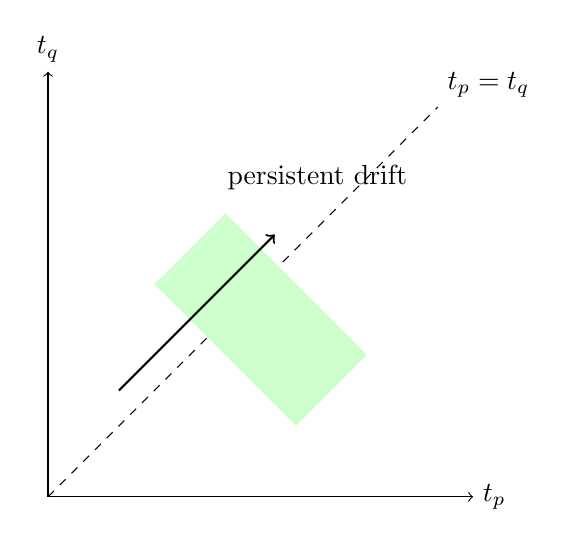
\begin{tikzpicture}[scale=0.9]

% Axes
\draw[->] (0,0) -- (6,0) node[right] {$t_p$};
\draw[->] (0,0) -- (0,6) node[above] {$t_q$};

% Diagonal
\draw[dashed] (0,0) -- (5.5,5.5) node[above right] {$t_p = t_q$};

% Drift region
\fill[green!20] (1.5,3) -- (2.5,4) -- (4.5,2) -- (3.5,1) -- cycle;

% Trajectory
\draw[thick,->] (1,1.5) -- (2,2.5) -- (3.2,3.7);

% Label
\node at (3.8,4.5) {persistent drift};

\end{tikzpicture}
\caption{Independent local time evolution allows relative timing differences
between agents to persist across interactions.}
\label{fig:persistent-drift}
\end{figure}

%---------------------------------------------------------------------------------

\subsection{Design choices and modelling rationale}
\label{subsec:ltn-design}

Local-timed negotiations combine ideas from negotiations and timed automata, but
the resulting model reflects a number of deliberate design choices.  We briefly
discuss the most important ones and contrast them with plausible alternatives.

\paragraph{Local clocks and delay vectors.}
Time elapse in LTNs is described by delay vectors $\Delta \in \Rpos^{P}$, rather
than by a single global delay.  This reflects the intended local-time semantics:
each agent progresses according to its own clock, and different agents may
accumulate time at different rates.  Using a single delay, as in timed automata,
would collapse the model back to a global-time view and eliminate the possibility
of drift between agents.

\paragraph{Reference clocks.}
Each agent $p$ is equipped with a reference clock $t_p$ that is never reset and
never appears in guards.  Reference clocks serve as a semantic device for tracking
the accumulated local time of an agent across the execution.  By excluding
reference clocks from guards, we ensure that agents cannot directly observe or
test global time; instead, comparisons between reference clocks are possible only
indirectly, via explicit synchronization.

\paragraph{Synchronization as a constraint.}
In LTNs, synchronization is expressed as the equality constraint
$t_p = t_q$ at synchronizing nodes, rather than as an instantaneous time jump or
reset.  Equality must be achieved by choosing appropriate local delays before the
action.  This makes synchronization an explicit modelling choice and separates
``time passing'' from ``time comparison'' in the semantics.

\paragraph{Node-based synchronization.}
Synchronization is associated with nodes (atomic negotiations) rather than with
outcomes.  This aligns with the interaction-centric nature of negotiations: timing
constraints are imposed at the level of joint interactions, not at the level of
local control-flow choices.

\paragraph{Local guards and resets.}
Guards and resets are local to each participating agent.  This prevents implicit
global coordination through shared clocks and ensures that all cross-agent timing
dependencies arise either from the negotiation structure itself or from explicit
synchronization nodes.

%---------------------------------------------------------------------------------

\section{Expressiveness}
\label{sec:ltn-expressiveness}

Here we understand the model better via two more examples.

\subsection{Causal Enforcement Through Synchronization}
\label{subsec:ltn-causal}

In global-time models, causality arises from control flow and shared clocks. LTNs add a new mechanism: \emph{using synchronization to force intermediate interactions}. An agent can be compelled to perform actions (accumulate local time) to align with a partner's reference clock.

\begin{example}[Forcing intermediate interactions via timing]
\label{ex:vendor}
Consider three agents: $p$, $q$, and a vendor $v$. Agent $p$ wants to ensure that $q$ has visited the vendor between their two meetings. Figure~\ref{fig:vendor} shows how this can be enforced using local clocks and synchronization.

\begin{figure}[t]
\centering
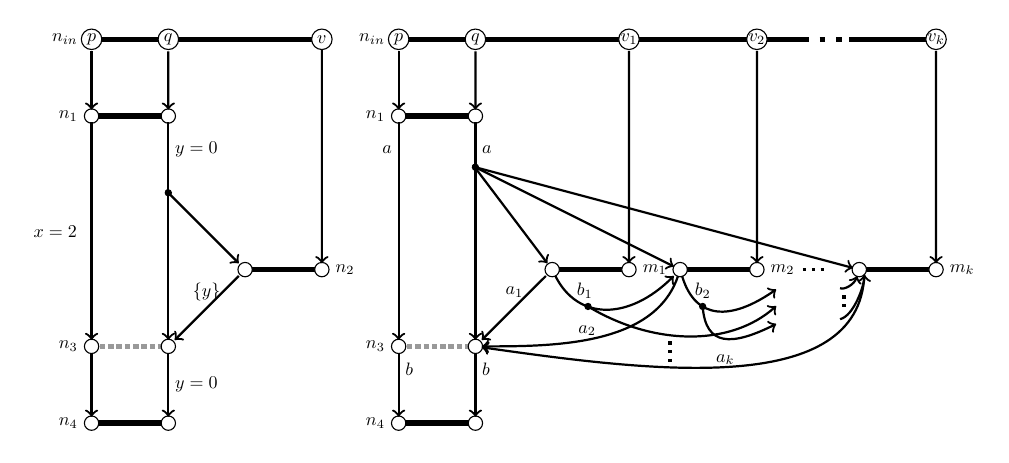
\begin{tikzpicture}[scale=0.65, every node/.style={transform shape}]

\begin{scope}[shift={(-6,0)}]
\begin{scope}[line width=2pt]
\draw (0.,0) node [left] {$n_{in}\,\,$} -- (4.5,0);
\draw (0,-1.5) node [black, left, opacity=1] {$n_1\,\,$} -- (1.5,-1.5);
\draw (3,-4.5)  -- (4.5,-4.5) node [right] {\,\,$n_2$};
\draw [densely dotted, opacity=0.4] (0,-6) node [black, left, opacity=1] {$n_3\,\,$} -- (1.5,-6);
\draw (0,-7.5) node [left] {$n_{4}\,\,$} -- (1.5,-7.5);
\end{scope}

\filldraw [fill=white]  (0,0)  circle (2mm) node 		(nip) {$p$};
\filldraw [fill=white]  (1.5,0)  circle (2mm) node 		(niq) {$q$};
\filldraw [fill=white]  (4.5,0)  circle (2mm) node 		(niv) {$v$};

\filldraw [fill=white]  (0,-1.5)  circle (1.4mm) node 	(n1p) {};
\filldraw [fill=white]  (1.5,-1.5)  circle (1.4mm) node (n1q) {};

\filldraw [fill=black]  (1.5,-3) circle (.6mm) node		(virt) {};

\filldraw [fill=white]  (3,-4.5)  circle (1.4mm) node 	(n21) {};
\filldraw [fill=white]  (4.5,-4.5)  circle (1.4mm) node (n2v) {};

\filldraw [fill=white]  (0,-6)  circle (1.4mm) node 	(n3p) {};
\filldraw [fill=white]  (1.5,-6)  circle (1.4mm) node 	(n3q) {};

\filldraw [fill=white]  (0,-7.5)  circle (1.4mm) node 	(nfp) {};
\filldraw [fill=white]  (1.5,-7.5)  circle (1.4mm) node (nfq) {};


\begin{scope}[thick,->]

\draw (nip) -- (n1p);
\draw (n1p) -- (n3p) node [midway, left, text width = 1cm] {$x=2$};
\draw (n3p) -- (nfp) node [midway, left] {};

\draw (niq) -- (n1q);
\draw (n1q) -- (n3q) node [very near start, right] {$y=0$};
\draw (virt) + (-.05,.05) -- (n21);
\draw (n21) -- (n3q) node [midway, above] {$\{y\}$};
\draw (n3q) -- (nfq) node [midway, right, text width = 1cm] {$y=0$};

\draw (niv) -- (n2v);

\end{scope}
\end{scope}

\begin{scope}[line width=2pt]
\draw (0.,0) node [left] {$n_{in}\,\,$} -- (7.9,0);
\draw (8.8,0) node [left] {} -- (10.5,0);
\draw (0,-1.5) node [black, left, opacity=1] {$n_1\,\,$} -- (1.5,-1.5);
\draw (3,-4.5)  -- (4.5,-4.5) node [right] {\,\,$m_1$};
\draw (5.5,-4.5)  -- (7,-4.5) node [right] {\,\,$m_2$};
\draw (9,-4.5)  -- (10.5,-4.5) node [right] {\,\,$m_k$};
\draw [densely dotted, opacity=0.4] (0,-6) node [black, left, opacity=1] {$n_3\,\,$} -- (1.5,-6);
\draw (0,-7.5) node [left] {$n_{4}\,\,$} -- (1.5,-7.5);
\end{scope}

\filldraw [fill=white]  (0,0)  circle (2mm) node 		(nip) {$p$};
\filldraw [fill=white]  (1.5,0)  circle (2mm) node 		(niq) {$q$};
\filldraw [fill=white]  (4.5,0)  circle (2mm) node 		(niv) {$v_1$};
\filldraw [fill=white]  (7,0)  circle (2mm) node 		(niv2) {$v_2$};
\filldraw [fill=white]  (10.5,0)  circle (2mm) node 		(nivk) {$v_k$};

\filldraw [fill=white]  (0,-1.5)  circle (1.4mm) node 	(n1p) {};
\filldraw [fill=white]  (1.5,-1.5)  circle (1.4mm) node (n1q) {};

\filldraw [fill=black]  (1.5,-2.5) circle (.6mm) node		(virt) {};

\filldraw [fill=white]  (3,-4.5)  circle (1.4mm) node 	(n21) {};
\filldraw [fill=white]  (4.5,-4.5)  circle (1.4mm) node (n2v) {};

\filldraw [fill=white]  (0,-6)  circle (1.4mm) node 	(n3p) {};
\filldraw [fill=white]  (1.5,-6)  circle (1.4mm) node 	(n3q) {};

\filldraw [fill=white]  (0,-7.5)  circle (1.4mm) node 	(nfp) {};
\filldraw [fill=white]  (1.5,-7.5)  circle (1.4mm) node (nfq) {};

\filldraw [fill=white]  (5.5,-4.5)  circle (1.4mm) node 	(v2q) {};
\filldraw [fill=white]  (7,-4.5)  circle (1.4mm) node (v2v) {};

\filldraw [white, fill=white]  (7.5,-4.8)  circle (1.4mm) node (virt2) {};
\filldraw [white, fill=white]  (8.5,-4.8)  circle (1.4mm) node (virt3) {};
\filldraw [white, fill=white]  (8.5,-5.5)  circle (1.4mm) node (virt8) {};

\filldraw [fill=black]  (3.7,-5.22)  circle (.6mm) node (virt4) {};
\filldraw [fill=black]  (5.94,-5.22)  circle (.6mm) node (virt5) {};

\filldraw [white, fill=white]  (7.5,-5.1)  circle (1.4mm) node (virt6) {};
\filldraw [white, fill=white]  (7.5,-5.5)  circle (1.4mm) node (virt7) {};

\filldraw [fill=white]  (9,-4.5)  circle (1.4mm) node 	(vkq) {};
\filldraw [fill=white]  (10.5,-4.5)  circle (1.4mm) node (vkv) {};

\begin{scope}[thick,->]

\draw (nip) -- (n1p);
\draw (n1p) -- (n3p) node [very near start, left] {$a$};
\draw (n3p) -- (nfp) node [near start, right, text width = 1cm] {$b$};

\draw (niq) -- (n1q);
\draw (n1q) -- (n3q) node [very near start, right] {$a$};
\draw (virt) + (-.05,.05) -- (n21);
\draw (n3q) -- (nfq) node [near start, right, text width = 1cm] {$b$};

\draw (niv) -- (n2v);

\draw (niv2) -- (v2v);
\draw (nivk) -- (vkv);

\draw (1.5,-2.5) -- (v2q);
\draw (1.5,-2.5) -- (vkq);

\draw (n21) -- (n3q) node [near start, left = 0cm] {$a_1$};

\end{scope}

\draw [line width=2pt, loosely dotted] (7.9,0)  -- (8.8,0) {};
\draw [very thick, dotted] (7.9,-4.5)  -- (8.4,-4.5) {};
\draw [very thick, dotted] (8.7,-5)  -- (8.7,-5.3) {};
\draw [very thick, dotted] (5.3,-5.9)  -- (5.3,-6.3) {};

\draw [thick,->] (n21) .. controls (3.5,-5.5) and(4.5,-5.5) .. (v2q) node [very near start, right = 0.1cm] {$b_1$};
\draw [thick,->] (v2q) .. controls (5.8,-5.5) and(6.5,-5.5) .. (virt2) node [very near start, right = 0cm] {$b_2$};
\draw [thick,->] (virt3) .. controls (8.7,-4.9) and (8.9,-4.8) .. (vkq);
\draw [thick,->] (virt8) .. controls (8.9,-5.4) and (9.1,-4.8) .. (9.1,-4.6);
\draw [thick,->] (v2q) .. controls (5,-6) and (3,-6) .. (n3q) node [midway, above left= -0.1cm] {$a_2$};
\draw [thick,->] (3.7,-5.22) .. controls (5,-6) and (6.5,-6) .. (virt6);
\draw [thick,->] (5.94,-5.22) .. controls (6,-6) and (6.5,-6) .. (virt7);
\draw [thick,->] (9.1,-4.6) .. controls (9,-7) and (5,-6.5) .. (n3q) node [midway, above left = -0.1cm] {$a_k$};;

\end{tikzpicture}
\caption{Vendor enforcement example. Nodes $n_1$ and $n_3$ are synchronizing (shown with dotted style). At $n_1$, outcome $a$ has guards $x = 2$ for $p$ and $y = 0$ for $q$. At $n_3$, outcome $b$ requires $y = 0$ for $q$. Synchronization forces $q$ to visit vendor $v$ at $n_2$ to accumulate the needed 2 time units. In the figure on the right, the $a$ transition has guards $x = m$ for $p$ and $y = 0$ for $q$. Each $b_i$ transition has a guard $y=1$ and a reset of $y$ to ensure exactly $1$ unit of time is spent in the nodes $m_i$ before outcomes $b_i$. The outcomes $a_i$ have a reset of $y$. The $b$ transition from $n_3$ has a guard $y=0$.}   
	\label{fig:vendor}
\end{figure}

\paragraph{Setup.} Agents $p$ and $q$ have local clocks $x$ and $y$ respectively. Nodes $n_1$ and $n_3$ are synchronizing. At $n_1$, outcome $a$ has guard $x = 2$ for $p$ and $y = 0$ for $q$.

\paragraph{What happens.} After outcome $a$ at $n_1$:
\begin{itemize}
\item Agent $p$ has advanced its reference clock by exactly 2 units (enforced by guard $x = 2$), so $t_p = 2$.
\item Agent $q$ has not advanced at all (guard $y = 0$), so $t_q = 0$.
\end{itemize}

Now both agents are ready at $n_3$ (control-flow wise), and $n_3$ is synchronizing. For outcome $b$ to occur at $n_3$:
\begin{itemize}
\item Synchronization requires $t_p = t_q$, but currently $t_p = 2$ and $t_q = 0$.
\item The guard at $b$ requires $y = 0$ for agent $q$. Since $y$ evolves with $t_q$, letting time elapse for $q$ would make $y > 0$, violating the guard.
\end{itemize}

\paragraph{The only solution.} Agent $q$ cannot simply wait—doing so would violate the guard $y = 0$. Instead, $q$ must:
\begin{enumerate}
\item Visit node $n_2$ (interaction with vendor $v$),
\item Spend exactly 2 time units there (advancing $t_q$ by 2),
\item Reset clock $y$ to zero when leaving $n_2$,
\item Return to $n_3$ with $t_q = 2$ and $y = 0$, satisfying both synchronization and the guard.
\end{enumerate}

This demonstrates \emph{causal enforcement}: the structure of timing constraints and synchronization forces $q$ to take a specific path through the negotiation. Agent $p$ can compel $q$ to perform intermediate interactions by setting up a timing mismatch that can only be resolved by those interactions.
\end{example}

\paragraph{Generalization.} This pattern extends to forcing $q$ to visit $m$ out of $k$ vendors, each requiring $1$ time unit. By setting $p$ delay to $m$ at $n_1$ and requiring $q$ to accumulate exactly $m$ time units before resynchronizing at $n_3$, we force $q$ to interact with at least $m$ vendors. This shows that LTNs can encode counting and comparison—foreshadowing undecidability.

\paragraph{Contrast with global time.} In networks of timed automata with global time, all clocks advance uniformly. One cannot create a situation where agent $p$ is "ahead" of agent $q$ in a way that forces $q$ to perform compensating actions. The local-time semantics is essential for this expressiveness.

%%%%

\subsection{Non-regular untimed languages}
\label{subsec:ltn-nonregular}

A classical fact about timed automata is that their untimed languages are
regular.  LTNs need not share this limitation.  The reason is that local drift
can encode a counter-like quantity, while synchronization can compare the values
accumulated by different agents.

\begin{example}[Generating $\{a^n b^n c \mid n \geq 0\}$]
\label{ex:anbn}
Consider the LTN in Figure~\ref{fig:abc} with two agents $p$ and $q$. Agent $p$ performs action $a$ repeatedly at node $n_1$, and agent $q$ performs action $b$ repeatedly at node $n_2$. Both can then synchronize at node $n_3$ to perform action $c$.

\begin{figure}[htb]
\centering
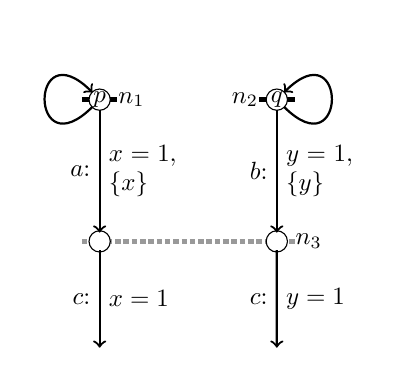
\begin{tikzpicture}[scale=0.9, every node/.style={transform shape}]

\begin{scope}[line width=2pt]
\draw (-.25,0) -- (0.25,0);
\draw (2.25,0) -- (2.75,0);
\draw [opacity=0.4, densely dotted] (-.25,-2) -- (2.75,-2);
\end{scope}

\filldraw [fill=white] (0,0) circle (1.5mm) node (pa) {$p$};
\filldraw [fill=white] (2.5,0) circle (1.5mm) node (qb) {$q$};
\filldraw [fill=white] (0,-2) circle (1.5mm) node (pc) {};
\filldraw [fill=white] (2.5,-2) circle (1.5mm) node (qc) {};

\node at (0.45,0) {$n_1$};
\node at (2.05,0) {$n_2$};
\node at (2.95,-2) {$n_3$};

\begin{scope}[thick,->]
\draw (pa) + (0,-.14) -- (pc) node [midway, left] {$a$:} node [midway, right, text width=1cm] {$x=1,$ $\{x\}$};
\draw (qb) + (0,-.14) -- (qc) node [midway, left] {$b$:} node [midway, right, text width = 1cm] {$y=1,$ $\{y\}$};
\draw (pc) -- (0,-3.5) node [midway, left] {$c$:} node [midway, right, text width=1cm] {$x=1$};
\draw (qc) -- (2.5,-3.5) node [midway, left] {$c$:} node [midway, right, text width=1cm] {$y=1$};
\draw (-0.1,-0.1) .. controls (-1,-1) and (-1,1) .. (-0.1,0.1);
\draw (2.6,-0.1) .. controls (3.5,-1) and (3.5,1) .. (2.6,0.1);
\end{scope}

\end{tikzpicture}
\caption{Non-regular untimed language. Each loop iteration of $a$ and $b$ takes exactly 1 time unit. Node $n_3$ is synchronizing with guards $x = 1$ and $y = 1$. This forces the number of $a$s to equal the number of $b$s before $c$ occurs.}
\label{fig:abc}
\end{figure}

\paragraph{Mechanism.} Both $p$ and $q$ start with reference clocks at zero. Each iteration of $a$ at $n_1$ takes exactly 1 time unit (guard $x = 1$, then reset $x$), advancing $t_p$ by 1. Similarly, each $b$ at $n_2$ advances $t_q$ by 1. The loops are concurrent—there's no ordering between $a$s and $b$s.

Node $n_3$ is synchronizing and requires:
\begin{itemize}
\item $t_p = t_q$ (synchronization condition),
\item $x = 1$ and $y = 1$ (guards at outcome $c$).
\end{itemize}

For these conditions to hold simultaneously:
\begin{itemize}
\item Both agents must have performed their last loop iteration exactly 1 time unit ago,
\item Both agents must have performed the same number of loop iterations (so $t_p = t_q$).
\end{itemize}

Therefore, if $p$ performs $n$ iterations of $a$ and $q$ performs $m$ iterations of $b$, action $c$ can occur if and only if $n = m$. The untimed language includes all words of the form $w \cdot c$ where $w$ has equal number of $a$ and $b$. Note that we can add another identical process with identical guards and which also time-synchronizes at $n_3$, and then the language would be beyond context-free.
\end{example}

\begin{proposition}
\label{prop:anbnc}
Let $L$ be the untimed outcome language of the gadget in
Figure~\ref{fig:abc}. Then
\[
L \cap a^*b^*c = \{a^n b^n c \mid n\ge 1\}.
\]
In particular, $L$ is not regular.
\end{proposition}

\begin{proof}
Consider a run whose untimed word belongs to $a^*b^*c$.  As long as the run
stays in the $a$-phase at $n_1$, only $p$ advances, and it does so by exactly
one time unit per $a$.  Once a $b$ is taken, $p$ moves to $n_3$ and can never
execute $a$ again, so the word has the form $a^n b^m c$ with $n,m\ge 1$.

At node $n_3$, outcome $c$ is synchronizing, so it requires $t_p=t_q$.  At
that moment, $p$ has accumulated exactly $n$ time units, one for each $a$, and
$q$ has accumulated exactly $m$ time units, one for each $b$.  Therefore $c$ is
enabled only if $n=m$.

Conversely, for every $n\ge 1$, the run can execute $a$ exactly $n$ times at
$n_1$, then take the first $b$ from $n_1$, then execute the $b$-loop at $n_2$
another $n-1$ times, and finally execute $c$ at the synchronizing node $n_3$.
Hence every word $a^n b^n c$ with $n\ge 1$ belongs to $L\cap a^*b^*c$.  The
displayed equality follows.  Since $a^*b^*c$ is regular and
$\{a^n b^n c \mid n\ge 1\}$ is not, $L$ itself cannot be regular.
\end{proof}

If one prefers the index set $n\ge 0$, it suffices to add a direct
$c$-transition from the initial node.  The essential point is unchanged:
synchronization compares quantities that were accumulated independently in local
time.

\paragraph{Why this matters.} This demonstrates that:
\begin{enumerate}
\item LTNs can encode \emph{counting} constraints across concurrent actions,
\item Synchronization acts as a \emph{comparison} operator between accumulated counts (via reference clocks),
\item The untimed behavior transcends finite-state structure—language-theoretically, LTNs are more powerful than timed automata.
\end{enumerate}

\begin{table}[t]
\centering
\begin{tabular}{ll}
\hline
\textbf{Feature} & \textbf{Modelling / expressive effect} \\ \hline
Local delay vectors & Independent progress and persistent drift \\
Reference clocks & Long-range timing information for each agent \\
Synchronizing nodes & Equality tests between local times \\
Local guards and resets & Counter-style timing patterns within a participant \\ \hline
\end{tabular}
\caption{Where the extra expressive power of LTNs comes from.}
\label{tab:ltn-expressiveness}
\end{table}

This expressiveness enables rich modelling but also implies undecidability, as we'll see next.

%---------------------------------------------------------------------------------
\begin{figure}[t]
\centering
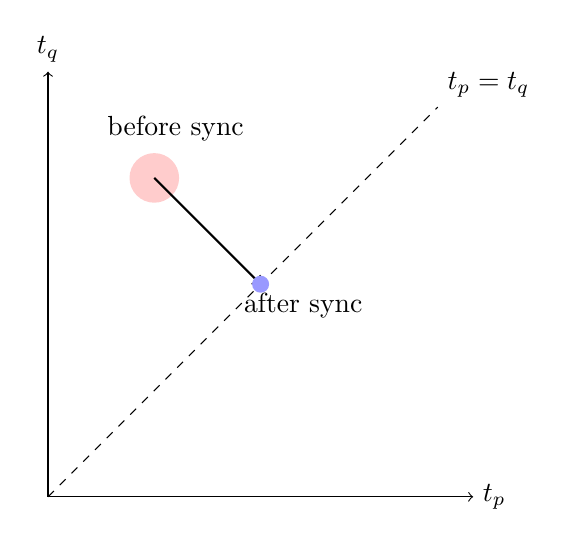
\begin{tikzpicture}[scale=0.9]

% Axes
\draw[->] (0,0) -- (6,0) node[right] {$t_p$};
\draw[->] (0,0) -- (0,6) node[above] {$t_q$};

% Diagonal
\draw[dashed] (0,0) -- (5.5,5.5) node[above right] {$t_p = t_q$};

% Pre-synchronization region
\fill[red!20] (1.5,4.5) circle (0.35);
\node at (1.8,5.2) {before sync};

% Arrow to diagonal
\draw[thick,->] (1.5,4.5) -- (3,3);

% Post-synchronization point
\fill[blue!40] (3,3) circle (0.12);
\node at (3.6,2.7) {after sync};

\end{tikzpicture}
\caption{A time-synchronizing interaction collapses relative timing differences,
allowing accumulated information to be compared or reset.}
\label{fig:selective-sync}
\end{figure}

%______________________________________________________________________________________________

\section{Undecidability of reachability}
\label{sec:ltn-undec}

\paragraph{Proof roadmap.}
The undecidability proof proceeds by a reduction from the halting problem of
$2$-counter machines.  The key idea is to encode counter values as differences
between reference clocks of carefully chosen agents.

Increment and decrement operations are implemented by allowing certain agents to
accumulate local time while others are forced to remain idle.  Zero-tests rely on
synchronizing nodes, which require equality of reference clocks and thus permit
the comparison of accumulated drift.  Unsynchronized nodes are essential for
allowing drift to grow without bound, while synchronized nodes are essential for
testing and transferring this information.

The construction alternates systematically between synchronized and
unsynchronized phases.  This interplay is what enables the simulation of
unbounded counters and ultimately yields undecidability of
location-reachability.

We now show that location-reachability for LTNs is undecidable.  The proof reduces
the halting problem of $2$-counter machines to reachability in an LTN.  The key
source of power is the unbounded drift between reference clocks of different agents,
together with the ability to impose synchronization at selected nodes.

\begin{theorem}
\label{thm:undecidability}
Location-reachability is undecidable for local-timed negotiations.
\end{theorem}

We prove the theorem by reduction from the halting problem for two-counter
machines.  Before giving the gadgets, it is useful to keep the following
dictionary in mind.

\begin{table}[t]
\centering
\begin{tabular}{ll}
\hline
\textbf{Counter machine object} & \textbf{LTN encoding} \\ \hline
Instruction label $\ell$ & Control node $n_\ell$ \\
Counter value $C_i=c_i$ & Drift $v(t_{p_i})-v(t_{q_i})=c_i$ \\
Increment of $C_i$ & Let $p_i$ alone elapse one unit of local time \\
Decrement / zero-test of $C_i$ & Compare $q_i$ with a frozen witness agent $r_i$ \\
Machine step & One \emph{big step} between encoding configurations \\ \hline
\end{tabular}
\caption{How the reduction encodes a two-counter machine inside an LTN.}
\label{tab:red-dictionary}
\end{table}

\subsection{Two-counter machines}
\label{subsec:2cm}

A \emph{two-counter machine} $M$ consists of labelled instructions $\ell:I$,
where $I$ is one of the following forms for some $i\in\{1,2\}$:
\begin{description}
\item[increment] $C_i{++}$, which increments $C_i$ and proceeds to instruction
      $\ell+1$;
\item[decrement] if $C_i>0$ then $C_i{--}$, which decrements $C_i$ and proceeds
      to $\ell+1$, and is otherwise blocked;
\item[jump-on-zero] if $C_i=0$ goto $\ell'$, which jumps to $\ell'$ when
      $C_i=0$ and otherwise proceeds to $\ell+1$.
\end{description}
A configuration of $M$ is a triple $(\ell,c_1,c_2)$, where $\ell$ is the
current instruction label and $c_1,c_2\in \mathbb N$ are the current counter
values.  The machine halts if it reaches its designated final instruction.

\subsection{Overview of the reduction}
\label{subsec:red-overview}

Given a two-counter machine $M$, we construct an LTN $\mathcal N_M$ with six
agents
\[
p_1,q_1,r_1,p_2,q_2,r_2.
\]
For each $i\in\{1,2\}$, the agents $p_i,q_i,r_i$ simulate counter $C_i$.  Their
local clocks are
\[
X_{p_i}=\{x_{p_i}\},\qquad
X_{q_i}=\{x_{q_i},x'_{q_i}\},\qquad
X_{r_i}=\{x_{r_i}\}.
\]
For every machine instruction label $\ell$, the negotiation contains a node
$n_\ell$ in which all six agents participate.

A configuration $(C,v)$ of $\mathcal N_M$ \emph{encodes}
$(\ell,c_1,c_2)$ if the following conditions hold:
\begin{enumerate}
\item $C(\alpha)=\{n_\ell\}$ for every agent $\alpha$;
\item all local clocks are $0$;
\item for each $i\in\{1,2\}$,
      \[
      v(t_{q_i})\le v(t_{r_i})\le v(t_{p_i});
      \]
\item for each $i\in\{1,2\}$,
      \[
      v(t_{p_i})-v(t_{q_i})=c_i.
      \]
\end{enumerate}

The initial configuration of $\mathcal N_M$ encodes the initial machine
configuration: all agents are ready at the node for the first instruction, and
all local and reference clocks are $0$.

A run segment that starts in one encoding configuration, ends in the next
encoding configuration, and has no intermediate configuration encoding a machine
state will be called a \emph{big step}.  The reduction is designed so that big
steps simulate exactly machine steps:
\begin{itemize}
\item if $(\ell,c_1,c_2)\to (\ell',c_1',c_2')$ is a machine transition, then
      every configuration encoding $(\ell,c_1,c_2)$ has a big step to some
      configuration encoding $(\ell',c_1',c_2')$;
\item conversely, every big step between encoding configurations corresponds to
      a valid machine transition.
\end{itemize}

The proof then concludes by designating a location that is reachable in
$\mathcal N_M$ iff the machine reaches its halting instruction.

Throughout the gadgets, guards of the form $x=0$ serve one simple but crucial
purpose: they prevent an agent from letting time pass unless the gadget
explicitly allows it.  Any unintended positive delay would violate such a guard
and block the run.

\subsection{Instruction gadgets}
\label{subsec:gadgets}

\begin{figure}[t]
\begin{center}
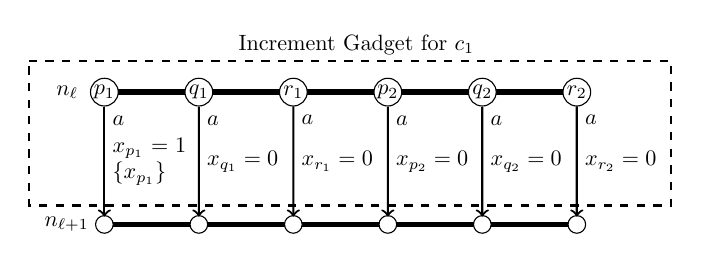
\begin{tikzpicture}[scale=0.8, every node/.style={transform shape}]

\begin{scope}[line width=2pt]
\draw (0,0) -- (7.5,0);
\draw (0,-2.1) -- (7.5,-2.1);
\end{scope}

\filldraw [fill=white]  (0,0)	  circle (2.2mm) node (nip1) [label={left:$n_{\ell}$}] {$p_1$};
\filldraw [fill=white]  (1.5,0)	  circle (2.2mm) node (niq1) {$q_1$};
\filldraw [fill=white]  (3,0)	  circle (2.2mm) node (nir1) {$r_1$};
\filldraw [fill=white]  (4.5,0)	  circle (2.2mm) node (nip2) {$p_2$};
\filldraw [fill=white]  (6,0)	  circle (2.2mm) node (niq2) {$q_2$};
\filldraw [fill=white]  (7.5,0)	  circle (2.2mm) node (nir2) {$r_2$};
\filldraw [fill=white]  (0,-2.1)	  circle (1.4mm) node (n2p1) [label={left:$n_{\ell + 1}$}] {};
\filldraw [fill=white]  (1.5,-2.1)	  circle (1.4mm) node (n2q1) {};
\filldraw [fill=white]  (3,-2.1)	  circle (1.4mm) node (n2r1) {};
\filldraw [fill=white]  (4.5,-2.1)	  circle (1.4mm) node (n2p2) {};
\filldraw [fill=white]  (6,-2.1)	  circle (1.4mm) node (n2q2) {};
\filldraw [fill=white]  (7.5,-2.1)	  circle (1.4mm) node (n2r2) {};

\begin{scope}[thick,->]
  \draw (nip1) -- node [very near start, right] {$a$} (n2p1)	 node [midway,right, text width=1.25cm] {$x_{p_1}=1$ $\{x_{p_1}\}$};
  \draw (niq1) -- node [very near start, right] {$a$} (n2q1)	 node [midway,right, text width=1.25cm] {$x_{q_1}=0$};
  \draw (nir1) -- node [very near start, right] {$a$} (n2r1)	 node [midway,right, text width=1.25cm] {$x_{r_1}=0$};
  \draw (nip2) -- node [very near start, right] {$a$} (n2p2)	 node [midway,right, text width=1.25cm] {$x_{p_2}=0$};
  \draw (niq2) -- node [very near start, right] {$a$} (n2q2)	 node [midway,right, text width=1.25cm] {$x_{q_2}=0$};
  \draw (nir2) -- node [very near start, right] {$a$} (n2r2)	 node [midway,right, text width=1.25cm] {$x_{r_2}=0$};
\end{scope}

\draw [dashed, thick] (-1.2,0.5) -- (9,0.5) -- (9,-1.8) -- (-1.2,-1.8) -- (-1.2,0.5);

\node at (4,.75) {Increment Gadget for $c_1$};
\end{tikzpicture}
\caption{Gadget for implementing increment instruction on $c_1$}
\label{fig:increment}
\end{center}
\end{figure}

\noindent \emph{Increment.} Assume an instruction $\ell: C_1 ++$ with $\ell$ not being the final instruction. The case with $C_2++$ is symmetric. Every configuration $(\ell, c_1, c_2)$ on executing this instruction goes to $(\ell + 1, c_1 + 1, c_2)$. Figure~\ref{fig:increment} shows the gadget for the increment instruction. All agents other than $p_1$ cannot elapse time due to the guard checking local clocks to $0$. Agent $p_1$ elapses
exactly one time unit, after which clock $x_{p_1}$ is reset.
It is easy to see that the configuration $(C', v')$ that results from $(C, v)$
encodes $(\ell', c_1 + 1, c_2)$. The big step $(C, v) \Rightarrow (C',v')$ is in fact a single transition. Both the properties are easily seen to be satisfied. 

\begin{lemma}
\label{lem:increment}
Assume that instruction $\ell$ of the counter machine is $C_1{++}$.  Every
successful big step of the gadget in Figure~\ref{fig:increment} from a
configuration encoding $(\ell,c_1,c_2)$ ends in a configuration encoding
$(\ell+1,c_1+1,c_2)$.  Conversely, every configuration encoding
$(\ell,c_1,c_2)$ has such a big step.
\end{lemma}

\begin{proof}
Let $(C,v)$ encode $(\ell,c_1,c_2)$, and write
\[
A:=v(t_{p_1}),\qquad B:=v(t_{q_1}),
\]
so that $A-B=c_1$.  Since every local clock is $0$ in an encoding
configuration, the zero guards on the edges for $q_1,r_1,p_2,q_2,r_2$ force
those five agents to take the unique outgoing action with delay $0$.  The guard
$x_{p_1}=1$ on the edge of $p_1$ forces $p_1$ to wait for exactly one time unit,
after which $x_{p_1}$ is reset.  Thus the gadget has a single possible big
step.

At the end of that step, all local clocks are again $0$.  The reference clocks
satisfy
\[
t'_{p_1}=A+1,\qquad t'_{q_1}=B,
\]
while $t_{r_1},t_{p_2},t_{q_2},t_{r_2}$ are unchanged.  Hence
\[
t'_{p_1}-t'_{q_1}=(A+1)-B=c_1+1,
\]
and the ordering constraints $t_{r_i}\le t_{q_i}\le t_{p_i}$ remain true for
both counters.  Therefore the target configuration encodes
$(\ell+1,c_1+1,c_2)$.  The converse direction is the same computation read
forwards: from any encoding configuration, the forced delay pattern described
above yields the required big step.
\end{proof}

\begin{figure}[t]
\centering
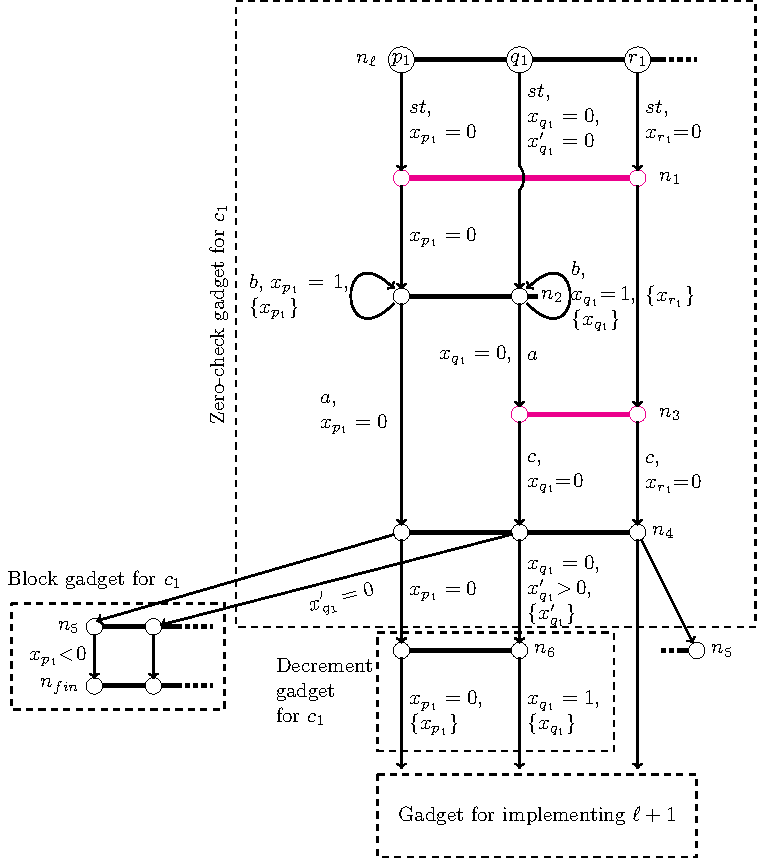
\includegraphics[width=.96\textwidth]{decrement-gadget.pdf}
\caption{Decrement gadget for counter $C_1$.  The highlighted horizontal bars
are the synchronizing nodes $n_1$ and $n_3$; the middle node $n_2$ is
deliberately unsynchronizing.  The gadget first copies the current reference
time of $p_1$ into the witness agent $r_1$, then advances $p_1$ and $q_1$
together until $q_1$ catches up with that frozen witness.  The branch taken
afterwards depends on whether a positive amount of time was needed.}
\label{fig:jump-decrement}
\end{figure}

\paragraph{Decrement.}
Now consider an instruction of the form ``if $C_1>0$ then $C_1{--}$''.
Suppose $(C,v)$ encodes $(\ell,c_1,c_2)$.  The counter value $c_1$ is stored as
the drift
\[
v(t_{p_1})-v(t_{q_1})=c_1.
\]
To test whether this difference is positive without destroying the encoding, the
gadget uses the auxiliary agent $r_1$ as a frozen witness.

The gadget works in three phases.

\emph{Phase 1: store the current reference time of $p_1$.}
Agents $p_1$ and $r_1$ pass through a synchronizing node while $p_1$ is
prevented from letting time elapse.  After this phase,
\[
t_{r_1}=t_{p_1},
\]
while $q_1$ remains unchanged.  The current value of the counter is therefore
remembered indirectly as the gap between $q_1$ and the witness $r_1$.

\emph{Phase 2: replay the difference.}
At an unsynchronized loop, agents $p_1$ and $q_1$ each advance by exactly one
unit per iteration, while $r_1$ is forced to stay put.  This preserves the
drift $t_{p_1}-t_{q_1}$, but moves $q_1$ steadily toward $r_1$.

\emph{Phase 3: test equality with the witness.}
The gadget now attempts to execute a synchronizing action between $q_1$ and
$r_1$.  This is possible exactly when $q_1$ has advanced by
\[
v(t_{p_1})-v(t_{q_1})=c_1
\]
units in Phase~2.  If the loop was executed too few or too many times, the
final synchronization is impossible and the run blocks.

At this point the auxiliary clock $x'_{q_1}$ records whether a positive amount
of time elapsed during Phase~2.  If the value is positive, the decrement branch
lets $q_1$ advance by one additional unit, thereby reducing the stored drift
from $c_1$ to $c_1-1$ and moving control to $n_{\ell+1}$.  If no time elapsed
in Phase~2, then the original counter value was $0$, and the gadget moves into
a blocking branch instead.

\begin{lemma}
\label{lem:decrement}
The decrement gadget for $C_1$ has a successful big step from a configuration
encoding $(\ell,c_1,c_2)$ iff $c_1>0$.  In that case the target configuration
encodes $(\ell+1,c_1-1,c_2)$.
\end{lemma}

\begin{proof}
Let $(C,v)$ encode $(\ell,c_1,c_2)$, and abbreviate
\[
A:=v(t_{p_1}),\qquad B:=v(t_{q_1}),\qquad R:=v(t_{r_1}),
\]
so that $A-B=c_1$ and $R\le B\le A$.  We reason only about the agents
$p_1,q_1,r_1$ shown in Figure~\ref{fig:jump-decrement}; the other three agents
are wired in parallel through zero-guard edges to the gadget for
$\ell+1$, so they never let time pass and preserve the value of $C_2$.

\smallskip
\noindent\emph{Phase 0: the forced start action.}
Because all local clocks are $0$ in an encoding configuration and the outgoing
edges of $n_\ell$ are guarded by
$x_{p_1}=0$, $x_{q_1}=0$, $x'_{q_1}=0$, and $x_{r_1}=0$, the outcome
$\mathsf{st}$ must be taken with delay $0$.  After this action, $p_1$ and
$r_1$ are at node $n_1$, while $q_1$ is at node $n_2$, and all clock values
are unchanged.

\smallskip
\noindent\emph{Phase 1: store the current time of $p_1$ in the witness $r_1$.}
The next relevant step is the synchronizing action at node $n_1$.  The guard
$x_{p_1}=0$ forbids any positive delay for $p_1$, so the only way to fire this
action is to let $r_1$ delay by exactly $A-R$ and keep $p_1$ fixed.  After the
action, $p_1$ moves to $n_2$ and $r_1$ to $n_3$, with
\[
t_{p_1}=A,\qquad t_{q_1}=B,\qquad t_{r_1}=A,
\]
and with
\[
x_{p_1}=x_{q_1}=x'_{q_1}=x_{r_1}=0.
\]
Thus the current reference time of $p_1$ is now frozen in the witness $r_1$.

\smallskip
\noindent\emph{Phase 2: replay the stored drift.}
At the unsynchronizing node $n_2$, the only progress-making action is the loop
$b$.  Its guards require $x_{p_1}=1$ and $x_{q_1}=1$, and the action resets
$x_{p_1}$ and $x_{q_1}$ but not $x'_{q_1}$.  Therefore, after exactly $k$
iterations of $b$,
\[
t_{p_1}=A+k,\qquad t_{q_1}=B+k,\qquad t_{r_1}=A,
\]
and
\[
x_{p_1}=x_{q_1}=0,\qquad x'_{q_1}=k,\qquad x_{r_1}=0.
\]
In particular, the drift $t_{p_1}-t_{q_1}$ is still $A-B=c_1$, while
$x'_{q_1}$ remembers how much local time has elapsed for $q_1$ since the start
of the gadget.

\smallskip
\noindent\emph{Phase 3: test equality with the witness.}
The action $a$ out of $n_2$ has guards $x_{p_1}=0$ and $x_{q_1}=0$, so it must
be taken with zero additional delay and moves $p_1$ to $n_4$ and $q_1$ to
$n_3$.  The following action $c$ is taken at the synchronizing node $n_3$ and
has guards $x_{q_1}=0$ and $x_{r_1}=0$.  Since these local guards already hold,
the synchronization requirement is the only nontrivial condition:
\[
t_{q_1}=t_{r_1}
\quad\Longleftrightarrow\quad
B+k=A
\quad\Longleftrightarrow\quad
k=A-B=c_1.
\]
Hence a successful continuation must execute the loop $b$ exactly $c_1$ times,
neither fewer nor more.

After the action $c$, the three reference clocks satisfy
\[
t_{p_1}=A+c_1,\qquad t_{q_1}=A,\qquad t_{r_1}=A,
\]
and all local clocks except $x'_{q_1}$ are $0$, while
\[
x'_{q_1}=c_1.
\]

If $c_1=0$, then only the branch guarded by $x'_{q_1}=0$ is enabled.  This
enters the block gadget.  The only outgoing edge there requires $x_{p_1}<0$,
which is impossible over nonnegative clock valuations.  Therefore no successful
big step can start from an encoding of $(\ell,0,c_2)$.

Assume now that $c_1>0$.  Then the branch guarded by
$x_{q_1}=0,\ x'_{q_1}>0,\ \{x'_{q_1}\}$ is enabled and moves the run to the
decrement sub-gadget.  From there, the only way back to an encoding
configuration is the branch in which $p_1$ takes its outgoing edge with
$x_{p_1}=0$ (hence lets no time pass) and $q_1$ takes its outgoing edge with
$x_{q_1}=1$ (hence lets exactly one time unit pass).  Both clocks are then
reset.  The resulting reference-clock values are
\[
t'_{p_1}=A+c_1,\qquad t'_{q_1}=A+1,\qquad t'_{r_1}=A.
\]
Therefore
\[
t'_{p_1}-t'_{q_1}=c_1-1,
\qquad
t'_{r_1}\le t'_{q_1}\le t'_{p_1},
\]
and all local clocks of $p_1,q_1,r_1$ are once again $0$.  Since the second
counter has been threaded through unchanged, the full target configuration
encodes $(\ell+1,c_1-1,c_2)$.

The converse direction has been proved along the way: any successful big step
must fire $c$, hence must use exactly $c_1$ loop iterations, and the guard on
$x'_{q_1}$ then forces the run into the decrement branch precisely when
$c_1>0$.  In that branch the target encoding computed above is the only
possible one.
\end{proof}


\begin{figure}[t]
\centering
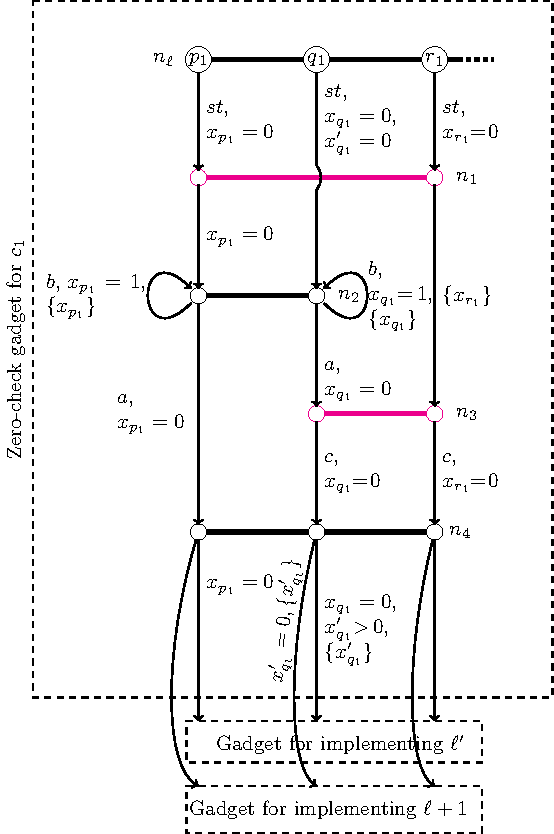
\includegraphics[width=.96\textwidth]{jump-gadget.pdf}
\caption{Jump-on-zero gadget for counter $C_1$.  It shares the same timing test
as the decrement gadget, but routes the zero case to instruction $\ell'$ and the
positive case to instruction $\ell+1$.}
\label{fig:jump}
\end{figure}

\paragraph{Jump-on-zero.}
The jump-on-zero gadget reuses the same three-phase timing test.  As before, it
first stores the current value of $t_{p_1}$ in the witness agent $r_1$, then
advances $p_1$ and $q_1$ together until $q_1$ meets the witness.  The auxiliary
clock $x'_{q_1}$ again records whether the replay phase consumed a positive
amount of time.

If $c_1=0$, then $q_1$ is already aligned with the witness after Phase~1, so
the replay phase needs zero iterations.  The auxiliary clock therefore records
the zero case, and the gadget branches to the target instruction $\ell'$ while
preserving the encoded drift.  If $c_1>0$, then the replay phase must take a
positive amount of time before the final synchronization becomes possible; in
that case the gadget branches to $n_{\ell+1}$, again without changing the
stored value of the counter.

\begin{lemma}
\label{lem:jump}
The jump-on-zero gadget for $C_1$ has a successful big step from a configuration
encoding $(\ell,c_1,c_2)$ to a configuration encoding $(\ell',c_1,c_2)$ iff
$c_1=0$, and to a configuration encoding $(\ell+1,c_1,c_2)$ iff $c_1>0$.
\end{lemma}

\begin{proof}
Let $(C,v)$ encode $(\ell,c_1,c_2)$, and write
\[
A:=v(t_{p_1}),\qquad B:=v(t_{q_1}),\qquad R:=v(t_{r_1}),
\]
so that $A-B=c_1$ and $R\le B\le A$.  The upper part of the jump gadget in
Figure~\ref{fig:jump} is identical to the zero-check part of the decrement
gadget.  Repeating the argument from the proof of Lemma~\ref{lem:decrement}, we
obtain the following facts.

First, the initial $\mathsf{st}$ action is forced with delay $0$ by the zero
guards on all local clocks.  Next, the synchronizing node $n_1$ copies the
current reference time of $p_1$ into the witness $r_1$ while keeping $p_1$
fixed, so after Phase~1 we have
\[
t_{p_1}=A,\qquad t_{q_1}=B,\qquad t_{r_1}=A
\]
and all local clocks are $0$.

Then the unsynchronizing loop $b$ at node $n_2$ may be executed $k$ times.  As
in the decrement gadget, after $k$ loop iterations we have
\[
t_{p_1}=A+k,\qquad t_{q_1}=B+k,\qquad t_{r_1}=A,
\]
\[
x_{p_1}=x_{q_1}=0,\qquad x'_{q_1}=k,\qquad x_{r_1}=0.
\]
The subsequent action $a$ is taken with zero additional delay, and the final
synchronizing action $c$ at node $n_3$ is enabled iff
\[
B+k=A,
\]
that is, iff $k=c_1$.  Hence any successful continuation reaches node $n_4$
with
\[
t_{p_1}=A+c_1,\qquad t_{q_1}=A,\qquad t_{r_1}=A,
\]
and with
\[
x_{p_1}=x_{q_1}=x_{r_1}=0,\qquad x'_{q_1}=c_1.
\]

At this point the gadget branches on the value of $x'_{q_1}$.
If $c_1=0$, then only the branch guarded by $x'_{q_1}=0$ is enabled.  This
branch resets $x'_{q_1}$ and routes the run to the gadget implementing
$\ell'$.  No additional delay is taken by $p_1,q_1,r_1$, so the reference-clock
values remain
\[
t'_{p_1}=A,\qquad t'_{q_1}=A,\qquad t'_{r_1}=A,
\]
and all local clocks are again $0$.  Therefore the target configuration encodes
$(\ell',0,c_2)$, which is the same as $(\ell',c_1,c_2)$ in this case.

If $c_1>0$, then only the branch guarded by
$x_{q_1}=0,\ x'_{q_1}>0,\ \{x'_{q_1}\}$ is enabled.  This branch also adds no
further local delay for $p_1,q_1,r_1$; it merely resets $x'_{q_1}$ and routes
the run to the gadget implementing $\ell+1$.  Hence the reference-clock values
remain
\[
t'_{p_1}=A+c_1,\qquad t'_{q_1}=A,\qquad t'_{r_1}=A,
\]
so that
\[
t'_{p_1}-t'_{q_1}=c_1,
\qquad
t'_{r_1}\le t'_{q_1}\le t'_{p_1}.
\]
All local clocks are again $0$, and the second counter is unchanged because the
agents $p_2,q_2,r_2$ are threaded through the branch with only zero-guard
transitions.  Thus the target configuration encodes $(\ell+1,c_1,c_2)$.

Conversely, the branch guards show that the jump target $\ell'$ is reachable
exactly when $x'_{q_1}=0$, i.e.\ exactly when $c_1=0$, and that the fall-through
target $\ell+1$ is reachable exactly when $x'_{q_1}>0$, i.e.\ exactly when
$c_1>0$.  These are the only successful big steps from an encoding
configuration.
\end{proof}


The gadgets for counter $C_2$ are symmetric.  By composing the appropriate
gadget after each instruction node $n_\ell$, the LTN $\mathcal N_M$ simulates
every step of $M$ and only those steps.

\begin{proof}[Proof of Theorem~\ref{thm:undecidability}]
For every machine instruction $\ell$, attach to the node $n_\ell$ the gadget of
the appropriate type: the increment gadget for instructions $C_i{++}$, the
decrement gadget for instructions ``if $C_i>0$ then $C_i{--}$'', and the
jump-on-zero gadget for instructions ``if $C_i=0$ goto $\ell'$''.  For
instructions on counter $C_2$, use the symmetric copies of the gadgets discussed
above.

By Lemma~\ref{lem:increment}, Lemma~\ref{lem:decrement}, and
Lemma~\ref{lem:jump}, the resulting negotiation $\mathcal N_M$ has the
following property: from every encoding configuration of a machine state
$(\ell,c_1,c_2)$, the successful big steps are exactly the encodings of the
machine successors of $(\ell,c_1,c_2)$.  In other words, machine steps and big
steps coincide on the encoding invariant.

Let $\ell_f$ be the halting instruction of $M$.  Add to the corresponding node
$n_{\ell_f}$ a fresh outcome $\mathsf{halt}$ whose local guard for each agent is
the appropriate zero guard on its local clock(s), whose reset set is empty, and
whose successor marking is an arbitrary sink marking.  In every encoding
configuration of the halting instruction all local clocks are already $0$, so
$\mathsf{halt}$ is enabled immediately.  Conversely, the location
$(n_{\ell_f},\mathsf{halt})$ cannot be executed from any encoding of a
non-halting instruction, because its source node is $n_{\ell_f}$.

We now prove the correctness of the reduction.  If
\[
(\ell_0,c_1^0,c_2^0)\to (\ell_1,c_1^1,c_2^1)\to \cdots \to (\ell_m,c_1^m,c_2^m)
\]
is a run of the machine, then repeated application of the three gadget lemmas
yields a sequence of big steps
\[
(C_0,v_0)\Rightarrow (C_1,v_1)\Rightarrow \cdots \Rightarrow (C_m,v_m)
\]
such that $(C_j,v_j)$ encodes $(\ell_j,c_1^j,c_2^j)$ for every $j$.  If
$\ell_m=\ell_f$, the additional outcome $\mathsf{halt}$ is enabled at
$(C_m,v_m)$, so the location $(n_{\ell_f},\mathsf{halt})$ is reachable in
$\mathcal N_M$.

Conversely, suppose $(n_{\ell_f},\mathsf{halt})$ is reachable in
$\mathcal N_M$.  By construction, the only incoming edges to an instruction node
$n_\ell$ are the final exits of instruction gadgets, and
Lemma~\ref{lem:increment}, Lemma~\ref{lem:decrement}, and
Lemma~\ref{lem:jump} show that each such exit re-establishes the encoding
invariant.  Hence any configuration from which $\mathsf{halt}$ can be executed
at $n_{\ell_f}$ is necessarily an encoding configuration of the halting
instruction.  Removing the final $\mathsf{halt}$ action, the remaining part of
the run decomposes into big steps between encoding configurations, and the
converse directions of the three gadget lemmas turn those big steps into a valid
run of the counter machine that reaches $\ell_f$.

Therefore $M$ halts iff $\mathcal N_M$ reaches the location
$(n_{\ell_f},\mathsf{halt})$.  Since the halting problem for two-counter
machines is undecidable, location reachability for LTNs is undecidable as well.
\end{proof}


The reduction also makes precise why the model crosses the decidability
boundary: local drift provides an unbounded numerical store, and synchronizing
nodes act as equality tests on that store.  Either ingredient alone is much less
dangerous; together they simulate counters.

% add the intuition diagram

%---------------------------------------------------------------------------------
\section{Summary and perspective}
\label{sec:summary-ch3}

This chapter introduced \emph{local-timed negotiations} (LTNs) as a real-time
extension of negotiations in which each agent carries its own set of local clocks,
and time elapses \emph{locally} (via delay vectors).  The semantics combines three
ingredients:

\begin{itemize}
  \item the negotiation-style control flow captured by markings (who is ready to
        participate in which node),
  \item local clock constraints (guards and resets attached to outcomes), and
  \item \emph{optional} explicit synchronization at selected nodes, expressed as the
        constraint that all participating agents have equal reference clocks.
\end{itemize}

We illustrated how LTNs model timing constraints between interactions using the
ATM example (Figure~\ref{fig:ATM}).  We then highlighted two expressiveness
phenomena that are characteristic of the local-time setting:
(i) synchronization can be used as a \emph{causal enforcement} mechanism, forcing
agents to perform intermediate interactions (Section~\ref{subsec:ltn-vendor}),
and (ii) the untimed outcome language of an LTN can be non-regular
(Section~\ref{subsec:ltn-nonregular}), in sharp contrast to timed automata where
the untimed language is always regular.

The main algorithmic message of the chapter is negative: we proved that
\emph{location-reachability is undecidable} for LTNs (Theorem~\ref{thm:undecidability})
by a reduction from halting of $2$-counter machines.  Conceptually, the reduction
pinpoints the source of power: reference clocks can drift arbitrarily, and
synchronizing nodes allow the system to \emph{compare} and \emph{transfer}
information encoded in those drifts.  In particular, the proof relies on a careful
interplay between synchronized nodes (where equality of reference clocks must be
met) and unsynchronized nodes (where agents can advance independently and thus
accumulate drift).

\smallskip
\noindent\textbf{Perspective.}
LTNs sit between two well-studied extremes.  On one hand, they inherit the
interaction-centric, partial-order flavour of negotiations; on the other hand,
they adopt a clock-based view of time as in timed automata, but without a global
time line.  This combination is expressive enough to model realistic timing
patterns (local deadlines, response windows, and time-bounded protocols), while
also making plain that \emph{unrestricted} local-time drift together with
\emph{explicit} synchronization yields a model beyond decidability for basic
reachability.

This motivates the rest of the thesis: to identify robust restrictions that
preserve the modelling advantages of LTNs but regain algorithmic tractability.
Two orthogonal axes stand out naturally from this chapter:
\begin{itemize}
  \item restricting (or eliminating) explicit synchronization, so that drift cannot
        be tested directly; and
  \item bounding the amount of drift that can accumulate (globally, per-agent, or
        per-cycle), so that comparisons do not simulate unbounded counters.
\end{itemize}
Understanding where decidability reappears along these axes also clarifies which
expressiveness features (e.g.\ enforcing intermediate interactions, or generating
non-regular untimed languages) survive in the restricted models, and which do not.

\smallskip
\paragraph{What causes undecidability?} The reduction pinpoints two features:
\begin{enumerate}
\item \textbf{Unbounded drift}: Reference clocks can diverge arbitrarily, encoding unbounded integer values (counter contents).
\item \textbf{Explicit synchronization}: Synchronizing nodes allow the system to test equality of reference clocks, enabling comparisons and conditional behavior based on encoded values.
\end{enumerate}

Removing or restricting either feature may recover decidability—this is the focus of Part~II.

%---------------------------------------------------------------------------------
\section{Coming next}
\label{sec:next-ch3}

This chapter concludes Part~I, where we introduced local-timed negotiations and
established that, in their full generality, even basic location-reachability is
undecidable (Theorem~\ref{thm:undecidability}).  The remainder of the thesis
(Part~II) is devoted to recovering decidability by identifying restrictions that
preserve the modelling advantages of LTNs while taming the two sources of
algorithmic hardness exposed by the reduction: \emph{unrestricted drift} between
local reference clocks and the ability to \emph{test} that drift via explicit
synchronization.

Part~II develops several decidable fragments along complementary axes:
\begin{itemize}
  \item \textbf{Extreme synchronization regimes:} we study the two endpoints where
        synchronization is either \emph{forbidden} (synchronization-free LTNs) or
        \emph{mandatory} at every interaction (always-synchronized LTNs), and
        analyze how these extremes change both expressiveness and the reachability
        problem.
  \item \textbf{Quantitative restrictions on drift:} we introduce drift-bounded
        variants that limit how far apart agents' reference clocks may deviate,
        yielding finite (or well-structured) symbolic state spaces.
  \item \textbf{Structural restrictions:} we consider communication/topological
        constraints on the underlying negotiation graph---for instance, connected
        communication patterns---and show how they can re-establish decidability
        even when clocks remain local.
  \item \textbf{Few-process settings:} we isolate the two-process case as a
        particularly informative boundary, where local time still matters but the
        concurrency structure becomes constrained enough to admit specialized
        algorithms.
\end{itemize}

\smallskip
\noindent\textbf{Immediate next chapter.}
We begin Part~II by focusing on the first axis above, namely the two extreme
synchronization regimes: \emph{synchronization-free} LTNs and \emph{always-synchronized}
LTNs.
